% Figure 3 of "The architecture of blockchain value: capabilities, pillars, and growth dynamics"
% (Papadogiannis, 2026, Front. Blockchain 9:1747512). Drawing code as in the author's manuscript.
% Compile with: pdflatex fig3_communication_structures.tex
\documentclass[border=6pt]{standalone}
\usepackage{amsmath, amssymb}
\usepackage{tikz}
\usetikzlibrary{positioning, shapes, arrows.meta, calc, backgrounds}
\begin{document}
\setlength{\tabcolsep}{10pt} % horizontal spacing between panels
\renewcommand{\arraystretch}{1.0}
\begin{tabular}{ccc}
% -------- Single-capability --------

\begin{tikzpicture}[scale=0.9, every node/.style={font=\small}]
  \node[draw, rounded corners=2pt, minimum width=2.4cm, minimum height=2.4cm] (box) {};
  \node[circle, draw, fill=gray!20, minimum size=1.2cm] at (0,0) {Service};
\end{tikzpicture}
&
% -------- Multi-capability (one bounded cluster) --------
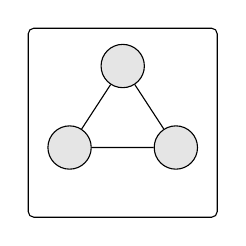
\begin{tikzpicture}[scale=0.9, every node/.style={font=\small}]
  \node[draw, rounded corners=2pt, minimum width=2.4cm, minimum height=2.4cm] (box) {};
  \node[circle, draw, fill=gray!20, minimum size=0.55cm] (m1) at (0,0.80) {};
  \node[circle, draw, fill=gray!20, minimum size=0.55cm] (m2) at (-0.75,-0.35) {};
  \node[circle, draw, fill=gray!20, minimum size=0.55cm] (m3) at (0.75,-0.35) {};
  \draw (m1)--(m2)--(m3)--(m1); % single bounded cluster
\end{tikzpicture}
&
% -------- Meta-capability (multiple clusters + clear cluster boundaries + bridges) --------
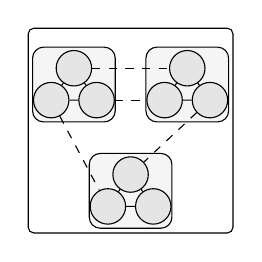
\begin{tikzpicture}[scale=0.9, every node/.style={font=\small}]
  % Outer environment
  \node[draw, rounded corners=2pt, minimum width=2.6cm, minimum height=2.6cm] (box) {};
  % --- Cluster A (top-left bubble) ---
  \begin{scope}
    \node[draw, rounded corners=4pt, fill=gray!8, minimum width=1.05cm, minimum height=0.95cm] (A) at (-0.80,0.65) {};
    \node[circle, draw, fill=gray!20, minimum size=0.45cm] (a1) at ($(A.center)+(0, 0.23)$) {};
    \node[circle, draw, fill=gray!20, minimum size=0.45cm] (a2) at ($(A.center)+(-0.32,-0.22)$) {};
    \node[circle, draw, fill=gray!20, minimum size=0.45cm] (a3) at ($(A.center)+(0.32,-0.22)$) {};
    \draw (a1)--(a2)--(a3)--(a1); % internal solid links
  \end{scope}
  % --- Cluster B (top-right bubble) ---
  \begin{scope}
    \node[draw, rounded corners=4pt, fill=gray!8, minimum width=1.05cm, minimum height=0.95cm] (B) at (0.80,0.65) {};
    \node[circle, draw, fill=gray!20, minimum size=0.45cm] (b1) at ($(B.center)+(0, 0.23)$) {};
    \node[circle, draw, fill=gray!20, minimum size=0.45cm] (b2) at ($(B.center)+(-0.32,-0.22)$) {};
    \node[circle, draw, fill=gray!20, minimum size=0.45cm] (b3) at ($(B.center)+(0.32,-0.22)$) {};
    \draw (b1)--(b2)--(b3)--(b1); % internal solid links
  \end{scope}
  % --- Cluster C (bottom-center bubble; suggests extensibility) ---
  \begin{scope}
    \node[draw, rounded corners=4pt, fill=gray!8, minimum width=1.05cm, minimum height=0.95cm] (C) at (0.00,-0.85) {};
    \node[circle, draw, fill=gray!20, minimum size=0.45cm] (c1) at ($(C.center)+(0, 0.23)$) {};
    \node[circle, draw, fill=gray!20, minimum size=0.45cm] (c2) at ($(C.center)+(-0.32,-0.22)$) {};
    \node[circle, draw, fill=gray!20, minimum size=0.45cm] (c3) at ($(C.center)+(0.32,-0.22)$) {};
    \draw (c1)--(c2)--(c3)--(c1); % internal solid links
  \end{scope}
  % --- Inter-cluster bridges (dashed) ---
  \draw[dashed] (a1) -- (b1);
  \draw[dashed] (a3) -- (b2);
  \draw[dashed] (b3) -- (c1);
  \draw[dashed] (a2) -- (c2);
\end{tikzpicture}
\\[-1mm]
\textbf{Single-capability} & \textbf{Multi-capability} & \textbf{Meta-capability}
\end{tabular}
\end{document}
